\chapter{Technical Approach}
In this chapter, we will explain the approaches employed in this work. Firstly, confronting with the limitations of concrete dropout, we propose another version of concrete dropout, which is called multiple dropout(multi-drop). Secondly, we introduce the modified architecture of ResNet50 in order to incorporate different inference techniques in BNN into this powerful feature extraction network. Thirdly, combination of BNN and CRF in this work is introduced, where CRF works as a post-processor to capture the relationship between random variables. Last but not least, we explain the approach combining aforementioned techniques for continuous learning in the last section.

\section{Multiple dropout}
From figure \ref{fig:dropout} and expression of approximate distribution in equation \ref{appro_dist_form}, we choose only one probability of Bernoulli distributed random variable for each layer, therefore random vector $\bld p_i = [p_i]^{D_{i-1}}$ for $i$-th layer, which stacks same value into a vector. While the dropout regularization term pushes the probability of Bernoulli to 0.5 to maximize its entropy, the expected likelihood term tries to increase the probability because decreasing probability will lead to a different model with lower capacity and thus low performance. An equilibrium state between them should be achieved in training. With concrete dropout introduced above, we could extend dropout for each hidden units instead of each layer(cf. figure \ref{fig:multi-drop}), which means random vector $\bld p_i = [p_i^k]_{k=1}^{D_{i-1}}$. While the first term in gradients computation stays the same, the second term should be modified to:
\begin{equation} 
\begin{aligned}\label{KL_grad_multi}
\frac{\partial KL(q_{\theta}(\bld \omega)||p(\bld \omega))}{\partial \theta} 
&\approx \frac{\partial \sum_{i=1}^{L}\lambda||\bld M_{i}||^{2}- \beta \mathcal H(\bld p_{i})}{\partial \theta}  \\
&= \frac{\partial}{\partial \theta} \big( \sum_{i=1}^{L}\lambda||\bld M_{i}||^{2}- \beta \sum_{k=1}^{D_{i-1}}(-p_i^k\text{log}p_i^k - (1-p_i^k)\text{log}(1-p_i^k))\big)
\end{aligned}
\end{equation}  

The reasons behind multi-drop are as following:
\begin{itemize}
\item to increase flexibility in tuning variational parameters. The tunability of parameter of Bernoulli random variable in the likelihood term is low because there is only single parameter controlling the entire layer. As is observed in the experiments(cf.figure \ref{fig:cdp_dropout2}), these parameters are always increased for each layer. The reason for this is probably that reducing it would lead to low capacity and thus low likelihood. 

\item the solution space of concrete dropout should be a subset of the solution space of multi-drop if all of them are reachable. Because if it's optimal to assign same probability for each hidden units, this can be recovered in training with multi-drop. Otherwise, other optimal solutions of assigning different probabilities to different hidden units could be considered.

\item last but not least, multi-drop can extend the flexibility and diversity of the dropout approximate distribution family by adding more parameters. Hence the truth posterior can be approximated by the approximate posterior better.
 
\end{itemize}


\begin{figure}[H]
	\begin{center}
		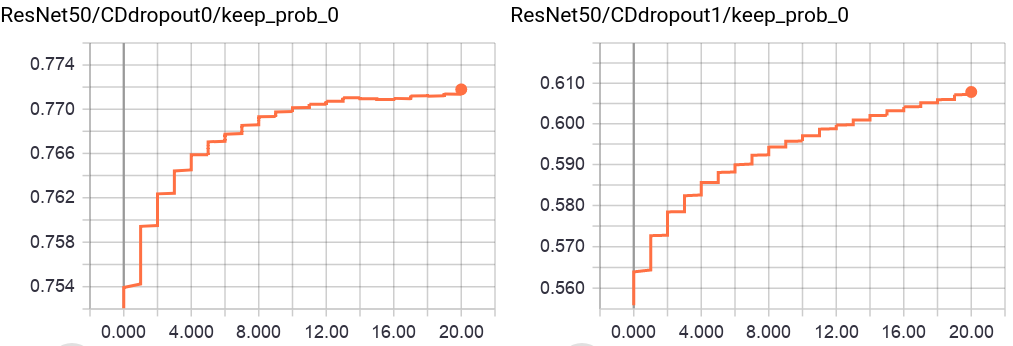
\includegraphics[height=4cm, width=11cm]{cdp_dropout1}	
		\caption{Changes of keep probability of the first two concrete dropout layers during training.}
		\label{fig:cdp_dropout1}
	\end{center}
\end{figure}
\begin{figure}[H]
	\begin{center}
		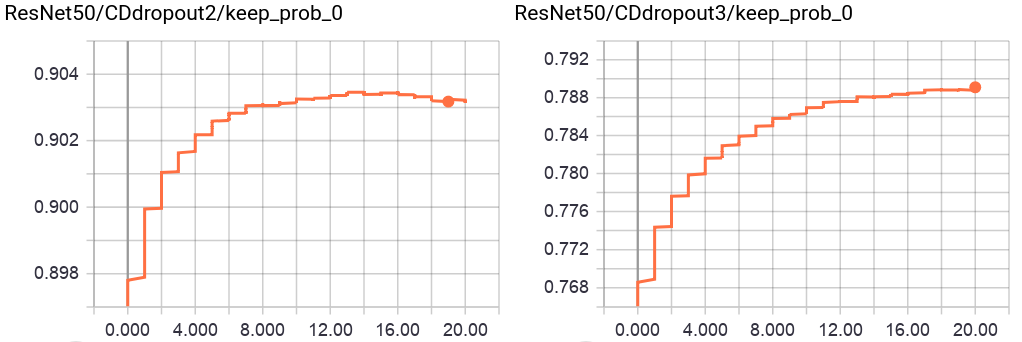
\includegraphics[height=4cm, width=11cm]{cdp_dropout2}	
		\label{fig:cdp_dropout2}
		\caption{Changes of keep probability of the last two concrete dropout layers during training.}
	\end{center}
\end{figure}
\begin{figure}[H]
	\begin{center}
		\centering
		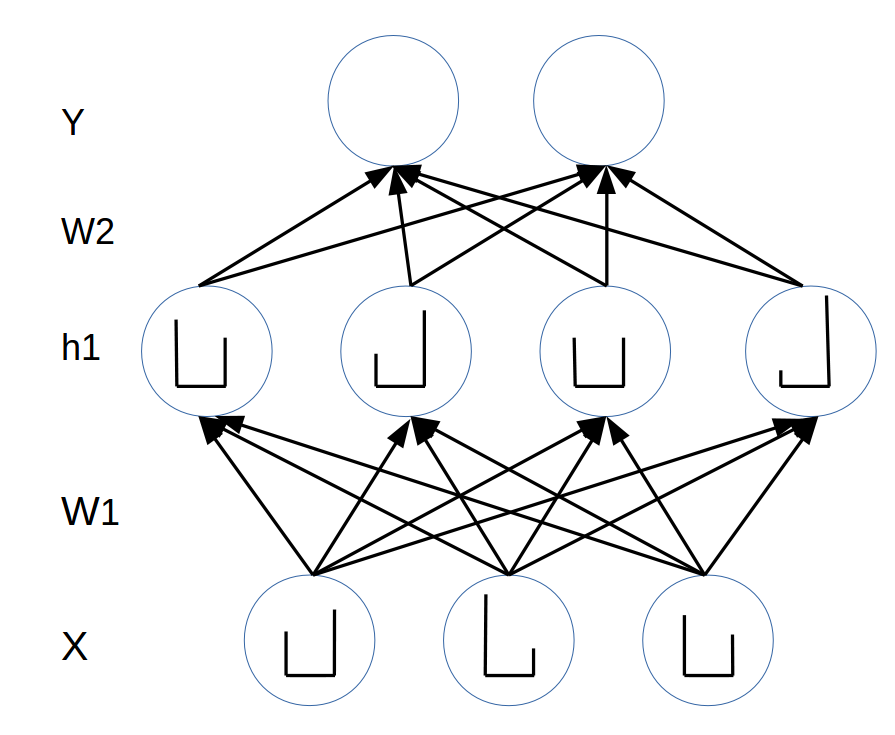
\includegraphics[width=11cm]{multi-drop}
		\caption{Different dropout rates for different hidden units in multi-drop.}		
		\label{fig:multi-drop}
	\end{center}
\end{figure}


\section{Modified network architecture}
After introducing dropout and concrete dropout variational inference, we will describe the modified network architecture in this subsection. The fundamental task in this work is object classification. We choose ResNet50\cite{he2016deep} pre-trained on ImageNet as backbone for fine-tuning because of its strong ability to learn powerful representation for images. However, there is no dropout in original version of ResNet50. If we want to employ dropout variational inference to obtain reliable uncertainty estimation, dropout should be inserted into the network. In this work, we add three fully connected layer with 1024 hidden units , which are initialized from scratch, before the output layer whose dimension needs to be set to the number of classes. Then we add concrete dropout at flatten layer, and these three new added fully connected layer, respectively.
There are three reasons why we modify the network in this way:
\begin{itemize}
	\item Inserting dropout in layers initialized with pre-trained weights will destroy pre-trained features. Because we initialize major part of network with pre-trained weights, hence it would lead to significant drop of performance after fine-tuning if we insert dropout into them. 
	\item According to the suggestions from \cite{srivastava2014dropout}, insertion of dropout reduces the capacity of the model and thus a model with	dropout should have larger capacity than one without dropout. Therefore we add three more fully connected layers to make sure that our model possesses large enough model capacity.
	\item As we have introduced in previous sub-sections, weights are major part of variational parameters. Therefore to have more weights can enhance the flexibility and capacity of approximate distribution family, which improves the quality of approximation.  
\end{itemize}

Figure \ref{fig:modified_net} shows the sketch of our modified network architecture. We can interpret major part of network, which do not have dropout inserted, as a deterministic feature extractor. Following this, there four layers with dropout inserted work as a probabilistic classifier. These four layers include one flatten layer with 2048 hidden units, and three fully connected layer with 1000 hidden units each. At the end, an output layer with size of number of categories is appended. The version of dropout inserted can be normal dropout, concrete dropout or multiple dropout. In this report, we only show results of concrete dropout and multiple dropout because normal dropout underperfroms when compared with them.   

In training, these two parts are trained together in order to achieve a better balance between uncertainty estimation and accuracy. As known to all, freezing feature extraction part can lead to worse performance, but it can also reduce the influence on predictive uncertainty from aleatoric uncertainty. To investigate this effect, we have done a ablation study which is shown in experiment part. In testing, we need to marginalize possible parameters according to posterior distribution. Layers with dropout should be turned on, sampled and run multiple times to perform Monte Carlo integration to approximate predictive distribution. The reduction of run time in testing can be achieved with different techniques, such as parallel computing or distillation. But this is out of the scope of this work.
\begin{figure}[H]
	\begin{center}
		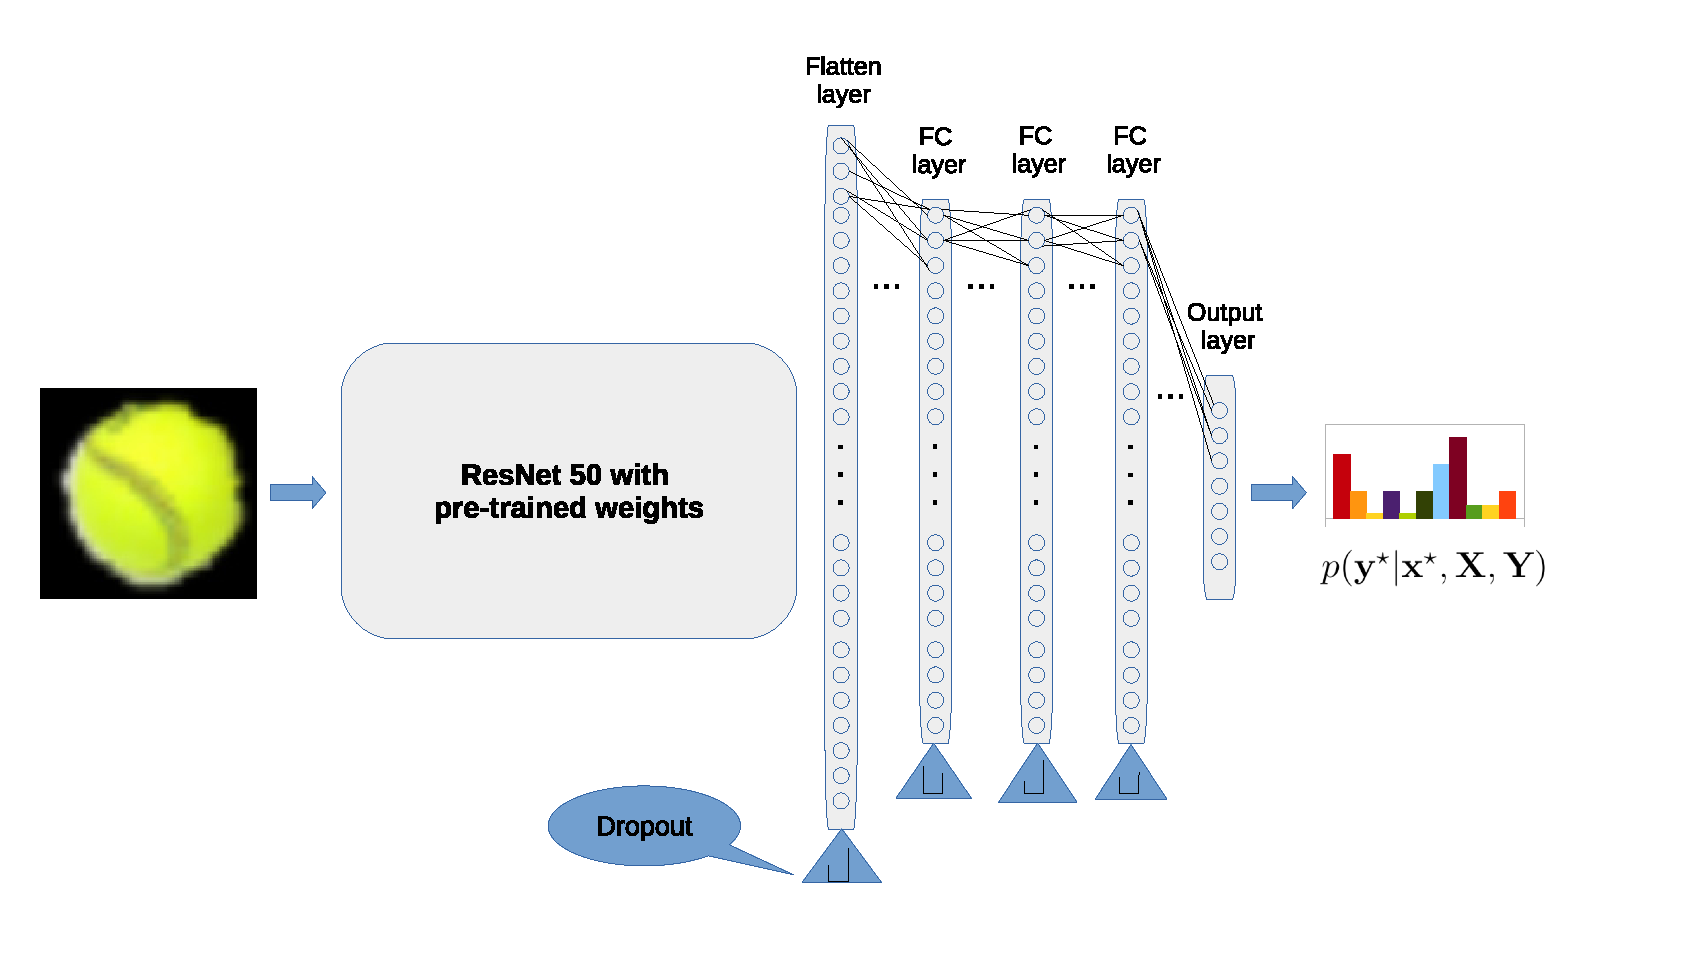
\includegraphics[height=8.5cm, width=15.5cm]{m_network}
		\caption{Modified network architecture of ResNet50.}		
		\label{fig:modified_net}
	\end{center}
\end{figure}

\section{Combination with CRF}\label{com_crf}
After employing Bayesian neural network, the model can provide more reliable uncertainty estimation in a probabilistic manner. In other words, the output distribution can bring more information than before. It would be better to make use of this information with another probabilistic model. In this work, we explore to combine output from BNN and relationship between objects in scene via CRF. In detail, we use output distribution from BNN for unary feature and binary co-occurrence matrix for pairwise feature (introduced in \ref{crf_def}). Figure \ref{fig:combined_crf} demonstrate the flow chart how BNN and CRF is combined together. As we can see, objects in one scene are firstly fed into BNN and their output distributions are fed into CRF as unary feature for each node. In the scene, their contextual relationship is represented by the binary co-occurrence matrix which is fed into CRF as pairwise feature. Then LBP is used to infer the marginal distribution of each node. 

One key factor in this case is that the pairwise feature is required to be designed by hand. The choice and design of it have significant impact on the improvement achieved by CRF. The information brought by pairwise feature should be complementary instead of contradictory to that of unary feature. Once this point is fulfilled, the more information unary feature has, the more improvement CRF can achieve.

 One thing worth noting, in experiment part, we test this approach only on T-LESS dataset. Because to construct scene for objects in WRGBD dataset is non-trivial. The reason for this is that most objects there have not only similar appearances but also similar contexts. Therefore it's hard to disambiguate miss-classification by incorporating their contextual information.
\begin{figure}[H]
	\begin{center}
		\includegraphics[height=8cm, width=15cm]{combined_crf}
		\caption{Combination of BNN and CRF.}		
		\label{fig:combined_crf}
	\end{center}
\end{figure}
\section{Approach for continuous learning}
With reliable uncertainty estimation, one of our goals is to enable the classifier or robot to learn continuously. The classifier should be introspective and express the confidence about its predictions. It's common that the test data in real environment does not have exactly same distribution as the training set, which induces a significant performance drop. In this situation, we expect our classifier to be able to adapt itself in real environment by fine-tuning itself with as little manual effort as possible. 

This idea is visualized in figure \ref{fig:con_learn}. The initialization phase includes training model with easily obtainable dataset, which can public or synthetic dataset. Before deploying in the real environment, there is an adaptation phase which makes use of the aforementioned techniques. In this phase, the classifier should be able to adapt itself to the objects in real environment by fine-tuning with dataset collected with as little manual effort as possible. If the relationship between objects in real environment is complementary to the discriminative classifier and can be encoded well, CRF can be employed to capture the relationship to improve the performance further (cf. section \ref{com_crf}). After that, the classifier is deployed to test data in real environment. In the experiment part, we evaluate this approach on both UniHB(WRGBD) and T-LESS(synthetic T-LESS).
\begin{figure}[H]
	\begin{center}
		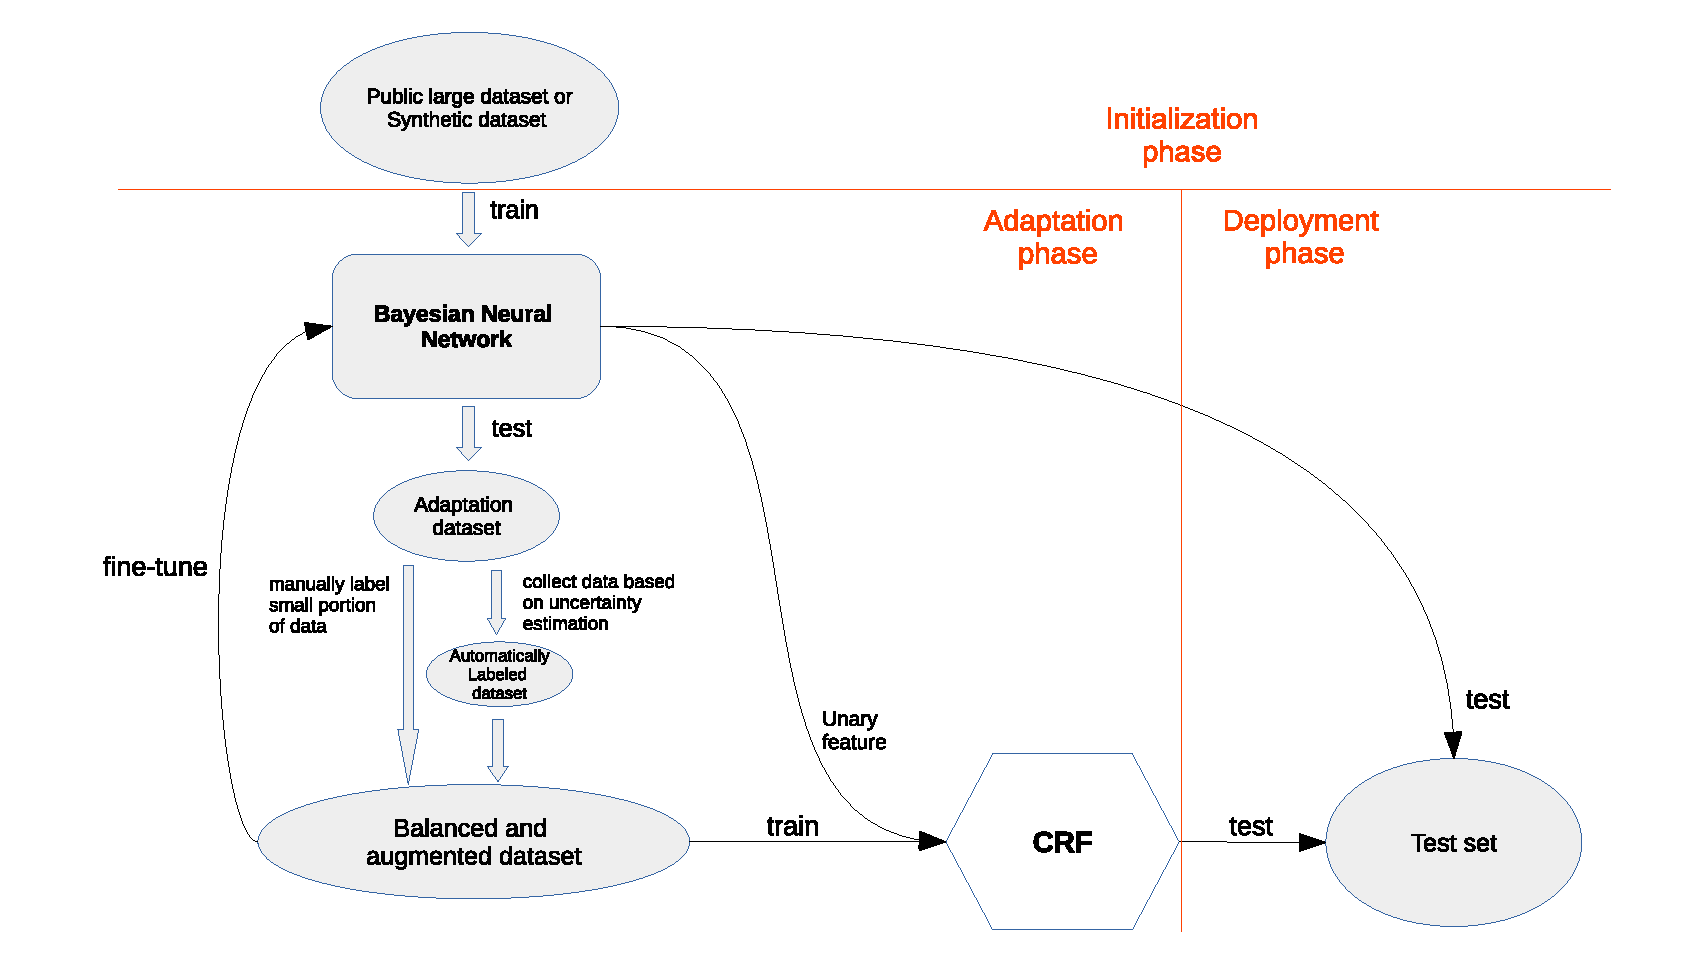
\includegraphics[height=10cm, width=16.5cm]{con_learn}
		\caption{Approach for continuous learning.}		
		\label{fig:con_learn}
	\end{center}
\end{figure}
